\documentclass[submission]{gmp2017}
%\documentclass{gmp2017}

\title{Parallel Quadtree Construction on Collections of Objects}

% Put your submission number here.
% This number will appear instead of authors and affiliations if the
% class option "submission" is active.
\SubNumber{19}

% Put the author names here.
% Use the second argument as a reference to the list of affiliations.
% No authors and affiliations will appear if the class option "submission"
% is active.
\author{Nathan Vollmer}{1}
\author{John Edwards}{1}

% Put the affiliations of the authors here.
\affiliation{1}{Department of Informatics and Computer Science, Idaho State University, USA}

%\usepackage{amsmath,amsthm,amsfonts,amscd,amssymb,amstext} 
\usepackage{amsmath,amsfonts,amscd,amssymb,amstext} 
\usepackage{mathrsfs}
				% Some packages to write mathematics.
\usepackage{overpic}
\usepackage{eucal} 	 	% Euler fonts
\usepackage{verbatim}      	% Allows quoting source with commands.
\usepackage{makeidx}       	% Package to make an index.
%\usepackage{citesort}         	% 
\usepackage{subfig}
\usepackage{graphicx}
\usepackage{url}		% Allows good typesetting of web URLs.
\usepackage{multirow}
%\usepackage[linesnumbered, noline]{algorithm2e}
%\usepackage[boxed, noline]{algorithm2e}
\usepackage[ruled]{algorithm2e}
\usepackage{booktabs}
\usepackage{tabularx}
\usepackage{array}
\usepackage{adjustbox}
\usepackage{color}
\usepackage{tikz}
% To balance the columns at the end
\usepackage{balance}
\usepackage[mediumspace,mediumqspace,Grey,squaren]{SIunits}
%\usepackage{draftcopy}		% Uncomment this line to have the
				% word, "DRAFT," as a background
				% "watermark" on all of the pages of
				% of your draft versions. When ready
				% to generate your final copy, re-comment
				% it out with a percent sign to remove
				% the word draft before you re-run
				% Makediss for the last time.
\usepackage[normalem]{ulem}

%\usepackage{cite}
\usepackage{balance}
\usepackage{color}

\definecolor{bostonuniversityred}{rgb}{0.8, 0.0, 0.0}
\definecolor{medblue}{rgb}{0.0, 0.0, 0.7}

%------------------------------------------------------------
% Custom commands
%------------------------------------------------------------
%\newcommand{\old}[1]{\textcolor{blue}{\sout{#1}}}
\newcommand{\old}[1]{}

%\newcommand{\red}[1]{\textcolor{red}{#1}}
\newcommand{\red}[1]{\textcolor{bostonuniversityred}{#1}}
\newcommand{\blue}[1]{\textcolor{medblue}{#1}}
\definecolor{light-gray}{gray}{0.75}
\newcommand{\gray}[1]{\textcolor{light-gray}{#1}}
%\newcommand{\red}[1]{#1}

%\newcommand{\reconstruct}{RECONSTRUCT\textsuperscript{\texttrademark}}
%\newcommand{\tm}{\textsuperscript{\texttrademark}}
\newcommand{\tm}{$^1$}
\newcommand{\addref}{\red{REF}}
\newcommand{\mathtext}[1]{\text{#1}}
\newcommand{\etal}{et al.\ }
\newcommand{\algorithmspace}{\vspace{8pt}}
\newcommand{\glfs}{\emph{glfs}}

\renewcommand{\vec}[1]{\mathbf{#1}}

\newcommand{\centercell}[1]{\multicolumn{1}{c}{#1}}
\newcolumntype{x}[1]{>{\centering\arraybackslash\hspace{0pt}}m{#1}}
\newcolumntype{y}[1]{>{\centering\arraybackslash\hspace{0pt}}m{#1\textwidth}}
\newcolumntype{M}{>{\centering\arraybackslash}m{1cm}}

\DeclareMathOperator*{\argmin}{arg\,min}
\DeclareMathOperator*{\argmax}{arg\,max}

\newcommand{\BigO}[1]{\ensuremath{\operatorname{O}\left(#1\right)}}
\newcommand{\centroid}{\mathscr{C}}
\newcommand{\iring}{\mathscr{R}}

% aligned
\renewcommand{\d}{\delta}
\newcommand{\vempty}{\mathscr{E}}
\newcommand{\e}{\epsilon}
\newcommand{\dist}{\mathtext{dist}}
\newcommand{\ball}{\mathscr{B}}


\newcommand{\hgt}{22mm}

%%--------------------------------------------------
%% Theorem environments (amsthm package required)
%%--------------------------------------------------
%% \theoremstyle{plain} %% This is the default
%\newtheorem{theorem}{Theorem}
%\newtheorem{lemma}{Lemma}
%\newtheorem{corollary}{Corollary}
%\newtheorem{conjecture}{Conjecture}
%\newtheorem{crit}{Criterion}
%\newtheorem{condition}{Condition}
%\newtheorem{fact}{Fact}

%\theoremstyle{definition}
%\newtheorem{defn}{Definition}[section]

%\theoremstyle{remark}
%\newtheorem{rem}{Remark}[section]
%\newtheorem*{notation}{Notation}

%\numberwithin{equation}{section}

%--------------------------------------------------
% Tight enumerations
%--------------------------------------------------
\newenvironment{tightenumerate}{
\begin{enumerate}
  \setlength{\itemsep}{1pt}
  \setlength{\parskip}{0pt}
  \setlength{\parsep}{0pt}
}{\end{enumerate}
}
\newenvironment{tightitemize}{
\begin{itemize}
  \setlength{\itemsep}{1pt}
  \setlength{\parskip}{0pt}
  \setlength{\parsep}{0pt}
}{\end{itemize}
}

%--------------------------------------------------
% Add figs to graphics path
%--------------------------------------------------
\graphicspath{{./}{./figs/}}

\newcolumntype{H}{@{}>{\lrbox0}l<{\endlrbox}}

%\newcommand{\container}[2]{container(#1, #2)}
\newcommand{\container}[1]{container(#1)}

\newcommand{\directAncestors}[1]{direct\_ancestors(#1)}

\newcommand{\lcp}{\textit{lcp}}

\newcommand{\shortcite}[1]{\cite{#1}}

\renewcommand{\paragraph}[1]{\noindent \textbf{#1}}



\usepackage[inline]{showlabels}

%-------------------------------------------------------------------------
\begin{document}

%\teaser{
%  \subfloat[][]{
%    \label{fig:gears1}
%    \begin{tikzpicture}
%      \node[anchor=south west,inner sep=0] at (0,0) {
%        \begin{tabular}[b]{c}
%          \includegraphics[height=0.8in]{gears-far1.png} \\
%          \includegraphics[height=0.8in]{gears-close1.png}
%        \end{tabular}
%      };
%      \draw[black,thick] (1.4,3.2) rectangle (2.0,3.6);
%      \draw[black,dashed] (1.4,3.6) -- (0.22,2.15);
%      \draw[black,dashed] (2.0,3.6) -- (2.95,2.15);
%      \draw[black,thick] (0.22,0.1) rectangle (2.95,2.15);
%    \end{tikzpicture}
%  }
%  \subfloat[][]{
%    \label{fig:gears}
%    \begin{tikzpicture}
%      \node[anchor=south west,inner sep=0] at (0,0) {
%        \begin{tabular}[b]{c}
%          \includegraphics[height=0.8in]{gears-far4.png} \\
%          \includegraphics[height=0.8in]{gears-close4.png}
%        \end{tabular}
%      };
%      \draw[black,thick] (1.3,3.1) rectangle (1.9,3.5);
%      \draw[black,dashed] (1.3,3.5) -- (0.22,2.15);
%      \draw[black,dashed] (1.9,3.5) -- (2.92,2.15);
%      \draw[black,thick] (0.22,0.1) rectangle (2.92,2.15);
%    \end{tikzpicture}
%  }
%  \hspace{3mm}
%  \subfloat[][]{
%    \label{fig:knife}
%    \includegraphics[trim=4cm 0cm 4cm 2.5cm, clip=true, height=1.4in]
%                    {knife-above/slice-00000.png}
%  }
%  \subfloat[][]{
%    \label{fig:knife2}
%    \includegraphics[trim=2mm 0cm 2mm 2cm, clip=true, height=1.4in]
%                    {knife-above/slice-00110.png}
%  }
%  \caption{Two example applications of the \red{approximated} generalized Voronoi diagram (GVD) computed by our novel, adaptive algorithm. Previous GVD methods require a gridded space of $2^{24}$ (gears dataset) and $2^{36}$ (knives dataset) voxels to resolve the closely spaced objects.
%    \protect\subref{fig:gears1} Two gears with regions of very tight spacing.
%    \protect\subref{fig:gears} The GVD of the gears model.  The surface is colored red in areas of very close tolerance.
%    \protect\subref{fig:knife} Three butter knives in a wood block.  To animate removal of the knives without intersecting the block requires extreme care because of close mesh spacing.
%    \protect\subref{fig:knife2} Intersection-free motion is guaranteed by computing motion vectors based on the GVD and allowing motion only within a Voronoi cell.
%  }
%  \label{fig:teaser}
%}
%
\maketitle

\begin{abstract}
We present a parallel quadtree algorithm that resolves between geometric objects. The quadtree has the property that no cell intersects more than one labeled object. A popular technique for discretizing space is to impose a uniform grid, an approach that is easily parallelizable, but this approach either fails because object separation isn't known a priori, or fails because the number of cells required to resolve closely spaced objects exceeds available memory. Previous parallel algorithms that are spatially adaptive, or that discretize finely in only where needed, either spawn kernels hierarchically, separate points only, or make no guarantees of object separation. Our 2D algorithm is the first to construct an object-resolving discretization that is hierarchical (saving memory) yet with a fully parallel approach (saving time). We describe our algorithm, derive the time complexity, demonstrate experimental results, and discuss extension to 3D. Our results show an order of magnitude improvement over the current state of the art.

%   Leave one blank line after the abstract, 
%   then add the subject categories according to the ACM Classification Index 
%   (see http://www.acm.org/class/1998/).

%\begin{classification} % according to http://www.acm.org/class/1998/
%  \CCScat{I.3.5}{Computer Graphics}{Computational Geometry and Object Modeling}{Boundary representations}
%  \CCScat{I.3.6}{Computer Graphics}{Methodology and Techniques}{Graphics data structures and data types}
%  %\CCScat{Computer Graphics}{I.3.3}{Picture/Image Generation}{Line and curve generation}
%\end{classification}

\end{abstract}

%-------------------------------------------------------------------------
% Body
%-------------------------------------------------------------------------

%-------------------------------------------------------------------------------
% introduction
%-------------------------------------------------------------------------------
\section{Introduction}
\label{sec:intro}
Constructing quadtrees on objects in an important task with applications in collision detection, distance fields, robot navigation, object description, and other applications. Quadtrees built on objects most often model the objects themselves, providing a space-efficient representation of arbitrarily complex objects. Our work however, centers on using quadtrees to separate, or resolve, collections of closely spaced objects, i.e., to construct a discretization such that no cell intersects more than one object. Using a quadtree, we can model the space between objects, the first step in constructing distance fields, detecting collisions, and computing the generalized Voronoi diagram. Modeling inter-object spacing is computationally straightforward when inter-object spacing is large compared to the world bounding box. Approaches typically involve a uniform grid of the space, which leads to efficient computation that often uses graphics processors.

Difficulties arise when spacing between objects is small relative to the size of the domain. An approach using a uniform grid would have excessive memory requirements in order to resolve between objects because the uniformly sized grid cell must be small enough to fit between objects at every location in the domain. Thus, an adaptive approach must be used for datasets of closely spaced objects. To our knowledge, only one algorithm \cite{edwards2015approximating} computes an adaptive data structure that fully resolves between objects without using unreasonable amounts of memory but does so in serial, with expected performance liabilities.

This work extends the work done by Edwards et al \cite{edwards2015approximating} by computing the quadtree in parallel with an algorithm targeted for the GPU. Our algorithm performs an order of magnitude faster than the previous work and will be an excellent base for later distance transform and generalized Voronoi diagram computation.

Our algorithm has three main components:

\begin{enumerate}
\item Construct an quadtree on object vertices using Karras' algorithm \cite{karras2012maximizing}
\item Detect quadtree cells that intersect more than one object, which we call ``conflict cells'' (contribution)
\item Subdivide conflict cells to resolve objects (contribution)
\end{enumerate}

Each step is done in parallel either on object vertices, object facets or quadtree cells.

%-------------------------------------------------------------------------------
% Related work
%-------------------------------------------------------------------------------
\section{Related work}

\paragraph{Serial} In an early work, Lavender \etal \shortcite{lavender1992voronoi} define and compute octrees over a set of solid models. 
% JME: note that in the Bastos work, ``reconstruction'' is reconstruction
% of the surface from the quadtree at rendering time.
Two seminal works build octrees on objects in order to compute the Adaptive Distance Field (ADF) on octree vertices.  Strain~\shortcite{strain1999fast} fully resolves the quadtree everywhere on the object surface, and Frisken \etal~\shortcite{frisken2000adaptively} resolve the quadtree fully only in areas of small local feature size.  Both approaches are designed to retain features of a single object rather than resolving between multiple objects, as is required for GVD computation. Boada \etal \shortcite{boada2002voronoi,boada2008approximations} use an adaptive approach to GVD computation, but their algorithm is restricted to GVDs with connected regions and is inefficient for polyhedral objects with many facets.  Two other works are adaptive \cite{teichmann1997polygonal,vleugels1998approximating} but are computationally expensive and are restricted to convex sites.

\paragraph{Parallel} Many recent works on fast quadtree construction using the GPU are limited to point sites \cite{bedorf2012sparse,karras2012maximizing,zhou2011data}. Kim and Liu's work~\shortcite{kim2014exact} is similar, computing the quadtree on the barycenters of triangles, giving an approximation of an object-resolving quadtree. Most quadtree approaches that support surfaces \cite{baert2013out,crassin2009gigavoxels,laine2011efficient,lefebvre2007compressed} are designed for efficient rendering, and actual construction of the quadtree is implemented on the CPU. Two works \cite{bastos2008gpu,park2010cuda} implement Adaptive Distance Fields in parallel on quadtrees but building the quadtree itself is done sequentially.  Yin \etal~\shortcite{yin2011fast} compute the octree entirely on the GPU using a bottom-up approach by initially subdividing into a complete quadtree, resulting in memory usage that is no better than using a uniform grid. We have found no GPU quadtree construction method that is fully adaptive and can resolve between objects.

%-----------------------------------------------------------
% Build quadtree
%-----------------------------------------------------------
\section{Algorithm}
\label{sec:algorithm}

We refer to quadtree leaf cells that intersect two or more objects as ``conflict cells.'' A necessary and sufficient condition for a quadtree to resolve objects is to have no conflict cells. Our approach to computing such a quadtree is to first build an initial quadtree using a set $S$ of point samples. We initialize $S$ to be the object vertices. We then detect conflict cells in parallel, followed by augmenting $S$ with sample points such that a subsequent quadtree built on $S$ resolves conflict cells. If $S$ changed, then we iterate.

Most of our algorithm is independent of dimension, and so we will use terms ``facet'' and ``octree'' (which lacks a dimension-independent term). The process of finding sample points to resolve conflict cells is limited to 2D in this paper, so for that section we will use ``line'' and ``quadtree''.

\subsection{Build initial octree}
\label{sec:build-initial-octree}
Our first step is to build an octree on the vertices. This step gives us our first approximation to our final octree. We use Karras' algorithm \cite{karras2012maximizing} which sorts the Morton codes of the vertices in parallel, then constructs the binary radix tree in parallel. With the binary radix tree, the quadtree can be constructed with a single parallel call. The strength of this algorithm lies in the fact that overall performance scales linearly with the number of cores, regardless of the distribution of points. That is, even if a large number of vertices are clustered in a small area, requiring deep quadtree subdivision, only a constant number of parallel calls need be made.

\subsection{Detect conflict cells}

Let the ``quadtree address'' refer to the unique ID of a quadtree cell $C$ found by concatenating the local addresses of its ancestors from Root to $C$, where the local address is the Morton code of a $2^{DIM}$ block of voxels. The address of the root cell is defined as the empty string. Figure \ref{fig:conflict-find-4} shows the address of each leaf cell in a quadtree.

We define a bounding cell (BCell) to be the smallest internal quadtree node which entirely contains a given facet. Given a facet defined by $n$ endpoints $P=\{p_1, p_2, \dots, p_n\}$, the quadtree address of the BCell is the longest common prefix of the Morton codes of the points in $P$. Figure \ref{fig:data-structures-1} gives the addresses of the BCells of the facets in figure \ref{fig:conflict-find-4}.

We begin by constructing an array \texttt{BCells} and sibling array \texttt{FacetMap} (see figure \ref{fig:data-structures-1}), which is done in parallel over all facets. Each facet $f$ computes the longest common prefix of its vertices and stores the result in \texttt{BCells[$f$]}.

Next we sort the \texttt{BCells} and \texttt{FacetMap} arrays on the \texttt{BCell} values using a parallel radix lexicographical sort (Figure \ref{fig:data-structures-2}). \texttt{BCells} array construction and sorting is done in parallel with the initial Karras octree construction.

\begin{figure}
  \centering
  \begin{tikzpicture}
    \node[anchor=south west,inner sep=0,outer sep=0] at (0,0) {
      \subfloat[][]{
        \label{fig:conflict-find-1}
        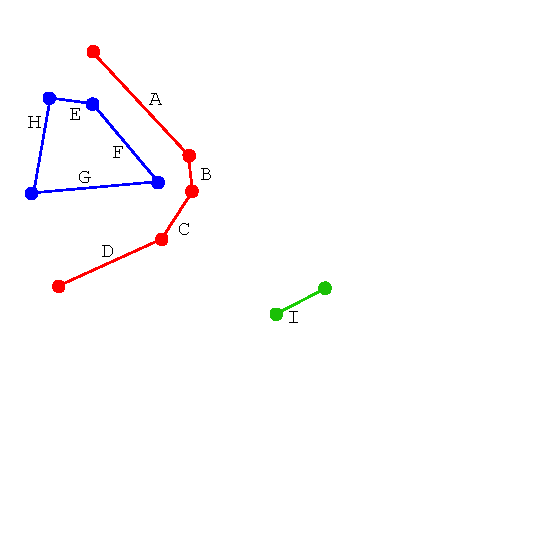
\includegraphics[width=0.22\columnwidth]{conflict-find-1.pdf} } \hfill
      \subfloat[][]{
        \label{fig:conflict-find-2}
        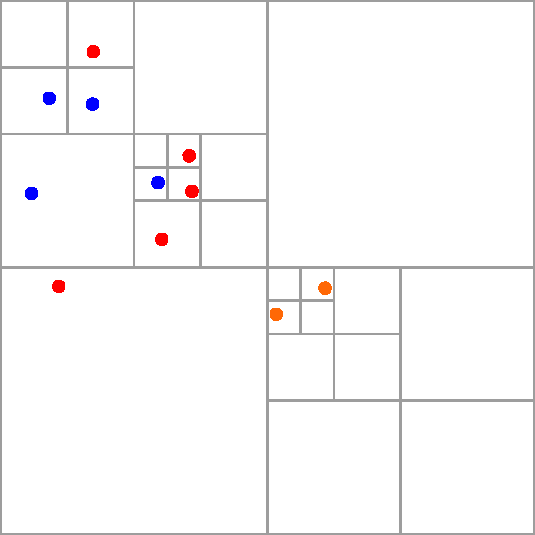
\includegraphics[width=0.22\columnwidth]{conflict-find-2.pdf} } \hfill
      \subfloat[][]{
        \label{fig:conflict-find-4}
        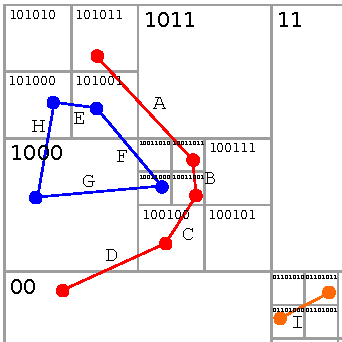
\includegraphics[width=0.22\columnwidth]{conflict-find-4.pdf} } \hfill
      \subfloat[][]{
        \label{fig:conflict-find-5}
        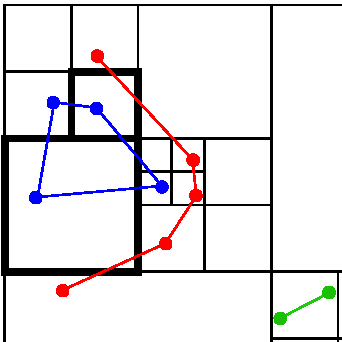
\includegraphics[width=0.22\columnwidth]{conflict-find-5.pdf} }
    };
    %\draw[red,ultra thick] (4.0,1.7) rectangle (6.55,4.2);
    \draw[red,thick] (4.0,1.7) rectangle (6.55,4.2);

    % lines
    % upper-right
    \draw[red,thin] (6.55,4.2) -- (11.8,4.2);
    % lower-left
    \draw[red,thin] (4.0,1.7) -- (8.0,0.3);

    %% curves
    %% upper-left
    %%\draw[red,thin] (4.0,4.2) to[out=10,in=170] (8.0,4.2);
    %% upper-right
    %\draw[red,thin] (6.55,4.2) to[out=10,in=170] (11.8,4.2);
    %% lower-left
    %\draw[red,thin] (4.0,1.7) to[out=-40,in=175] (8.0,0.3);

    \draw[red,thick] (8.0,0.3) rectangle (11.8,4.2);
  \end{tikzpicture} \\
      \subfloat[][]{
        \label{fig:conflict-find-6}
        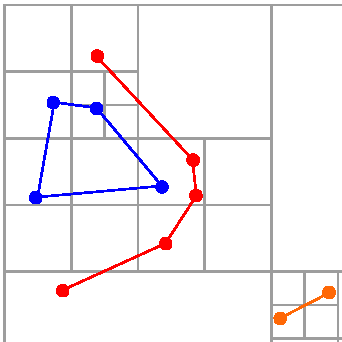
\includegraphics[width=0.22\columnwidth]{conflict-find-6.pdf} } \hfill
      \subfloat[][]{
        \label{fig:data-structures-1}
        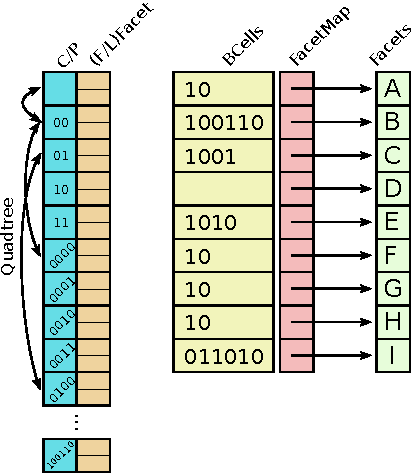
\includegraphics[width=0.22\columnwidth]{data-structures-1.pdf} } \hfill
      \subfloat[][]{
        \label{fig:data-structures-2}
        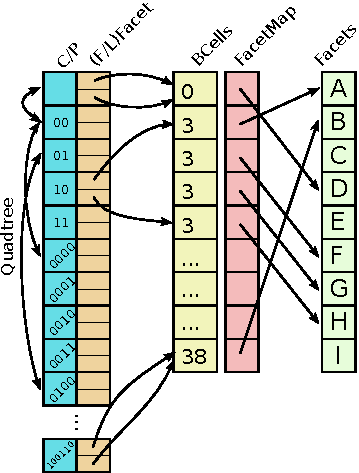
\includegraphics[width=0.22\columnwidth]{data-structures-3.pdf} } \hfill
      \subfloat[][]{
        \label{fig:data-structures-3}
        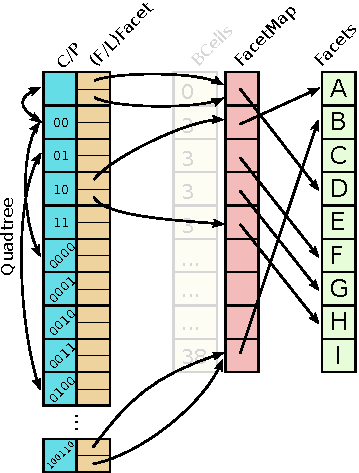
\includegraphics[width=0.22\columnwidth]{data-structures-4.pdf} }
  \caption{
    \protect\subref{fig:conflict-find-1} We have three objects, blue, red, and green with facets labeled A-I.
    \protect\subref{fig:conflict-find-2} We construct an initial quadtree on the vertices using Karras' algorithm.
    \protect\subref{fig:conflict-find-4} Zoomed-in view of the boundary cell (BCell) computation for each facet. These pairs are given in figure \protect\subref{fig:data-structures-1}.
    \protect\subref{fig:conflict-find-5} Conflict cells, which intersect more than one object, are highlighted.
    \protect\subref{fig:conflict-find-6} The new quadtree after conflict resolution.
    \protect\subref{fig:data-structures-1} The bounding cells (BCells) are stored in an array initially sorted on facet index (letters are used here for clarity). The quadtree array elements are structures which store child and parent pointers (``C/P'' in the figure).
    \protect\subref{fig:data-structures-2} We sort the BCells array using a parallel radix sort on BCell address for fast indexed access. We then, in parallel on each element of the BCells array, store the BCells/FacetMap indices of the first and last facets in a given octree cell in \texttt{FFacet} and \texttt{LFacet}, respectively.
\protect\subref{fig:data-structures-3} For a given octree cell, we can find all contained facets for use in algorithm \ref{alg:find-conflict-cells}.
  }
  \label{fig:conflict-find}
\end{figure}

\begin{figure}
  \label{fig:scc-sort}
\end{figure}

Then we use the \texttt{BCells} array and octree data structure to find the conflict cells using algorithm \ref{alg:find-conflict-cells}. We process each leaf cell $L$ in parallel (line \ref{alg:L}). We set $L$'s color to $-1$ (uninitialized). We then investigate each ancestor $A$ of $L$ (line \ref{alg:A}). We find the ancestors using the \texttt{Parent} field in the octree data structure. Using the \texttt{FFacet} and \texttt{LFacet} fields, we find, respectively, the first and (inclusive) last of possibly multiple facets bounded by $A$ (line \ref{alg:i}). We use the \texttt{FacetMap} array to find all facets bounded by bounding cell $A$ (line \ref{alg:f}). Any facet $f$ for which $A$ is the bounding cell could potentially intersect the leaf cell $L$. We test for intersection between $f$ and $L$ and store the first two facets of differing color (lines \ref{alg:7}-\ref{alg:16}). If at the conclusion of execution $L$.color is equal to $-2$ then $L$ is a conflict cell and must be resolved.

\algorithmspace
\begin{algorithm}
  \DontPrintSemicolon
  \LinesNumbered
  \KwIn{Quadtree}
  \BlankLine
  \ForPar{leaf cell $L$}{ \label{alg:L}
    $L$.color = -1\;
    \ForEach{cell $A$ in \directAncestors{$L$}}{  \label{alg:A}
      \ForEach{i in \{FFacet[A]$\dots$LFacet[A]\}}{ \label{alg:i}
%      i := Quadtree[$A$].Facets\; \label{alg:i}
%      \While{BCells[i].Cell\_ID = Address($A$)}{
%        $f$ := Facets[BCells[i].Facet\_idx]\; \label{alg:f}
        $f$ := Facets[FacetMap[i]]\; \label{alg:f}
        \If{$f$ intersects $L$}{ \label{alg:7}
          \If{$L$.color == -1} {
            $L$.color = $f$.color\;
            $L$.facet[0] = $f$\;
          }
          \ElseIf{$L$.color $\ne$ $f$.color} {
            $L$.color = -2\;
            $L$.facet[1] = $f$\;
          }
        } \label{alg:16}
      }
    }
  }
\caption{FIND\_CONFLICT\_CELLS}
\label{alg:find-conflict-cells}
\end{algorithm}
\algorithmspace

\subsection{Resolve conflict cells}

\begin{figure}
  \centering
  \subfloat[][]{
    \label{fig:conflict-resolution-x}
    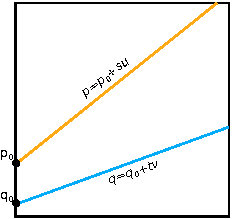
\includegraphics[width=0.24\columnwidth]{conflict-resolution-x.pdf} }
  \subfloat[][]{
    \label{fig:conflict-resolution-even}
    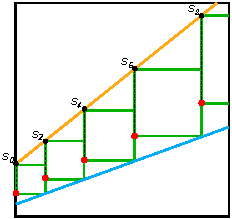
\includegraphics[width=0.24\columnwidth]{conflict-resolution-even.pdf} }
  \subfloat[][]{
    \label{fig:conflict-resolution-all}
    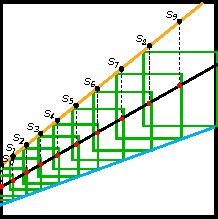
\includegraphics[width=0.24\columnwidth]{conflict-resolution-all.pdf} }
  \subfloat[][]{
    \label{fig:conflict-resolution-octree}
    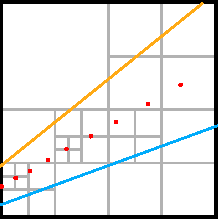
\includegraphics[width=0.24\columnwidth]{conflict-resolution-octree.pdf} } \\
  \subfloat[][]{
    \label{fig:conflict-resolution-adjacent-even}
    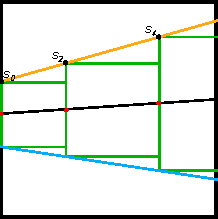
\includegraphics[width=0.24\columnwidth]{conflict-resolution-adjacent-even.pdf} }
  \subfloat[][]{
    \label{fig:conflict-resolution-adjacent-all}
    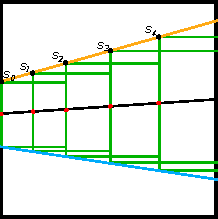
\includegraphics[width=0.24\columnwidth]{conflict-resolution-adjacent-all.pdf} }
  \caption{
    \protect\subref{fig:conflict-resolution-x} A conflict cell with two lines from different objects.
    \protect\subref{fig:conflict-resolution-even} Fitting boxes such that any box intersecting both lines contains at least one sample (red dots).
    \protect\subref{fig:conflict-resolution-even} Fitting boxes such that any box intersecting both lines contains at least two samples. This ensures that an quadtree built from the samples using Karras' algorithm (panel \protect\subref{fig:conflict-resolution-octree}) will have no leaf cells that intersect both lines, ensuring that the new quadtree is locally free of conflict cells.
  }
  \label{fig:conflict-resolution}
\end{figure}

We present a conflict cell resolution algorithm for pairs of lines in 2D. For a conflict cell $C$ our approach is to find sample points inside the cell such that no leaf cells in a quadtree constructed over the sample points intersect both lines. In this section we derive equation \eqref{eqn:num-samples} which computes the number of samples required to resolve the cell, and equation \eqref{eqn:sample} which computes the samples themselves. The power of our approach lies in the fact that both expressions are closed-form and neither one is iterative, so we can evaluate the first in parallel over leaf cells and the second in parallel over all samples to compute.

To resolve a conflict cell $C$, we consider pairs of lines of differing labels that intersect $C$. Figure \ref{fig:conflict-resolution-x} shows two lines

\begin{align}
q(t) &= q = q_0 + tv \label{eqn:q} \\
r(f) &= r = r_0 + fw \label{eqn:r}
\end{align}
along with a line
\begin{align}
p(s) &= p = p_0 + su \label{eqn:p}
\end{align}
that bisects $q$ and $r$. Our strategy will be to sample points $P$ on $p(s)$ (figure \ref{fig:conflict-resolution-octree}) such that an quadtree built on $S \cup P$ will completely ``separate'' $q$ and $r$, i.e., no descendent cell of $c$ will intersect both $q$ and $r$. We do this by ensuring that $P$ is sampled such that every box that intersects both $q$ and $r$ also intersects at least two points in $P$. Because Karras' algorithm guarantees that every leaf cell intersects at most one point, we know that no leaf cell will intersect $q$ and $r$ and thus no leaf cell will be a conflict cell. We will find a series of boxes such that each box's left-most intersection with $p(s)$ is a sample point meeting the above criterion.

We consider only cases where the slope of $p$ is in the range $0 \le m \le 1$. All other instances can be transformed to this case using rotation and reflection. We begin by fitting the smallest box centered on a point $p$ that intersects both $q$ and $r$. We break the problem into two cases: the \textit{opposite} case (see Figure \ref{fig:conflict-resolution-even}) is where $w^y > 0$, so each box intersects $q$ and $r$ at its top-left and bottom-right corners, respectively. The \textit{adjacent} case (see Figure \ref{fig:conflict-resolution-adjacent-even}) is where $w^y < 0$, so the line intersections are adjacent at the top-left and bottom-left corners of the box.

\subsubsection{Finding $a(s)$ -- \textit{opposite} case}

Given a point $p(s)$, we wish to find $a=a(s)$, which will give us the starting $x$ coordinate for the next box. Consider the top-left corner of the box $q(t(s))=q(t)$ and the bottom-right corner $r(f(s))=r(f)$.

Because $p^x(s)=q^x(t)$,
\begin{equation}
t = \frac{p^x(s)-q_0^x}{v^x} = \frac{p_x^x-q_0^x+su^x}{v^x} \label{eqn:t}
\end{equation}
Because our boxes are square,
\begin{equation}
r(f) = r_0+fw = q_0+tv+a\begin{bmatrix}1\\-1\end{bmatrix} \label{eqn:ro}
\end{equation}
From \eqref{eqn:ro},
\begin{align}
f &= \frac{1}{w^y}(q_0^y+tv^y-a-r_0^y) \label{eqn:f} \\
a &= r_0^x+fw^x-q_0^x-tv^x \label{eqn:a1o}
\end{align}
Substituting equations \eqref{eqn:t} and \eqref{eqn:f} into equation \eqref{eqn:a1o} and solving for $a$,
\begin{equation}
a(s) = \hat{\alpha}_o s + \hat{\beta}_o \label{eqn:ao}
\end{equation}
where
\begin{equation}
\hat{\alpha}_o = \frac{u^x|w \times v|}{v^x(w^x+w^y)}
\end{equation}
and
\begin{equation}
\hat{\beta}_o = \frac{|w \times v|(p_0^x-q_0^x) + v^x(|r_0 \times w| + |w \times q_0|)}{v^x(w^x+w^y)}
\end{equation}

\subsubsection{Finding $a(s)$ -- \textit{adjacent} case}

Consider the top-left corner of the box $q(t(s))=q(t)$ and the bottom-left corner $r(f(s))=r(f)$. $r(f)$ is now defined as
\begin{equation}
r(f) = r_0+fw = q_0+tv+a\begin{bmatrix}0\\-1\end{bmatrix} \label{eqn:ra}
\end{equation}
Equations \eqref{eqn:t} and \eqref{eqn:f} remain the same while \eqref{eqn:a1o} becomes
\begin{equation}
0 = r_0^x+fw^x-q_0^x-tv^x \label{eqn:a1a}
\end{equation}
Substituting equations \eqref{eqn:t} and \eqref{eqn:f} into equation \eqref{eqn:a1a} and solving for $a$,
\begin{equation}
a(s) = \hat{\alpha}_a s + \hat{\beta}_a \label{eqn:aa}
\end{equation}
where
\begin{equation}
\hat{\alpha}_a = \frac{u^x}{v^xw^x}
\end{equation}
and
\begin{equation}
\hat{\beta}_a = \frac{w^x(p_0^x-q_0^x)+|w \times q_0| + |r_0 \times w|}{w^x}
\end{equation}


%
%
%Because $p^x(s)=q^x(t)$,
%\begin{equation}
%t = \frac{p^x(s)-q_0^x}{v^x} = \frac{p_x^x-q_0^x+su^x}{v^x} \label{eqn:t}
%\end{equation}
%Because our boxes are square,
%\begin{equation}
%r(f) = r_0+fw = q_0+tv+a
%\begin{bmatrix}
%1\\-1
%\end{bmatrix}
%\label{eqn:r}
%\end{equation}
%From \eqref{eqn:r},
%\begin{align}
%f &= \frac{1}{w^y}(q_0^y+tv^y-a-r_0^y) \label{eqn:f} \\
%a &= r_0^x+fw^x-q_0^x-tv^x \label{eqn:a1}
%\end{align}
%Substituting equations \eqref{eqn:t} and \eqref{eqn:f} into equation \eqref{eqn:a1} and solving for $a$,
%\begin{equation}
%a = \alpha s + \beta
%\end{equation}
%where
%\begin{equation}
%\alpha = \frac{u^x|w \times v|}{v^x(w^x+w^y)}
%\end{equation}
%and
%\begin{equation}
%\beta = \frac{|w \times v|(p_0^x-q_0^x) + v^x(|r_0 \times w| + |w \times q_0|)}{v^x(w^x+w^y)}
%\end{equation}
%
%Consider a box with edge length $a_0$ centered on a point $p_0 \in p$. We first find $p$, which is the line that is equidistant from $q$ and $r$ along the diagonal vector $\gamma = (1, -1)$. Given some point $q(t)$,
%\begin{equation}
%q_0+tv + \lambda\gamma = r_0+fw \\
%\end{equation}
%Solving for $\lambda$,
%\begin{align}
%f &= \frac{1}{w^y}(q_0^y+tv^x-\lambda-r_0^y) \\
%\lambda &= r_0^x + fw^x-q_0^x-tv^x \\
%        &= r_0^x+\frac{w^x}{w^y}(q_0^y+tv^y-\lambda-r_0^y) - q_0^x-tv^x \\
%        &= \frac{1}{w^x+w^y}(r_0^xw^y+q_0^yw^x-r_0^yw^x-q_0^xw^y+t(v^yw^x-v^xw^y)
%\end{align}
%The vector $u = p - p_0$. We obtain $p$ from $q(0)$, by finding $\lambda/2$.
%\begin{align}
%p = q(0) + \frac{\lambda}{2}\gamma
%\end{align}
%We get $p_0$ by finding the intersection between the two lines. If they are parallel then we find two points $p$ using $q(0)$ and $q(1)$.
%
%To find $a$,
%\begin{align} 
%p^x-\frac{a}{2} &= q^x \\
%p^y+\frac{a}{2} &= q^y
%\end{align}
%Substituting equation \eqref{eqn:q},
%\begin{align} 
%t = \frac{p^x-a/2-q_0^x}{v^x} \\
%t = \frac{p^y+a/2-q_0^y}{v^y}
%\end{align}
%which leads to
%\begin{align} 
%\frac{p^x-a/2-q_0^x}{v^x} &= \frac{p^y+a/2-q_0^y}{v^y}
%\end{align}
%Solving for $a$,
%\begin{align}
%\label{eqn:plain_a}
%a &= \frac{2(p^xv^y-q_0^xv^y-p^yv^x+q_0^yv^x)}{v^x+v^y}
%\end{align}
%$a$ is a parametric function in $s$, so using equations \eqref{eqn:plain_a} and \eqref{eqn:p},
%\begin{align}
%a(s) &= \frac{2((p_0^x+su^x)v^y-q_0^xv^y-(p_0^y+su^y)v^x+q_0^yv^x)}{v^x+v^y} \\
%     &= s\frac{2(u^xv^y-u^yv^x)}{v^x+v^y} + \frac{2(p_0^xv^y-q_0^xv^y-p_0^yv^x+q_0^yv^x)}{v^x+v^y} \label{eqn:a}
%\end{align}
%Figure \ref{fig:conflict-resolution-even} shows that we will find a series of points $P=p(s_i)$ such that
%\begin{equation}
%p^x(s_i) = p^x(s_{i-2})+a(s_{i-2}) \label{eqn:p_s}
%\end{equation}
%Using equations \eqref{eqn:p}, \eqref{eqn:a} and \eqref{eqn:p_s},
%\begin{align}
%p_0^x+s_iu^x = p_0^x+s_{i-2}u^x+s_{i-2}\frac{2(u^xv^y-u^yv^x)}{v^x+v^y} + \frac{2(p_0^xv^y-q_0^xv^y-p_0^yv^x+q_0^yv^x)}{v^x+v^y}
%\end{align}
%Solving for $s_i$,
%\begin{equation}
%\label{eqn:si_rec}
%s_i = s_{i-2}\alpha + \beta
%\end{equation}
%where
%\begin{align}
%%\alpha &= \frac{u^xv^x+3u^xv^y-2u^yv^x}{u^x(v^x+v^y)}
%\alpha &= 1+\frac{2(u^xv^y-u^yv^x)}{u^x(v^x+v^y)} \\
%\beta &= \frac{2(p_0^xv^y-q_0^xv^y-p_0^yv^x+q_0^yv^x)}{u^x(v^x+v^y)}
%\end{align}

\subsubsection{Sampling}
In both the \textit{opposite} and the \textit{adjacent} cases, $a(s)$ is of the form $a(s) = \hat{\alpha} s + \hat{\beta}$. We now use $a(s)$ to construct a sequence of values $S = \{s_0, s_1, s_2, \dots, s_n\}$ that meet our sampling criterion. We first construct the even samples (see Figures \ref{fig:conflict-resolution-even} and \ref{fig:conflict-resolution-adjacent-even}). Given a starting point $p(s_0)$,
\begin{equation}
p^x(s_{i+2}) = p^x(s_i) + a(s_i)
\end{equation}
Substituting in equations \eqref{eqn:p} and \eqref{eqn:ao}/\eqref{eqn:aa},
\begin{equation}
p_0^x + s_{i+2}u^x = p_0^x + s_i + \hat{\alpha} s_i + \hat{\beta}
\end{equation}
Solving for $s_{i+2}$ gives the recurrence relation
\begin{equation}
s_{i+2} = \alpha s_i + \beta \label{eqn:recurrence}
\end{equation}
where
\begin{equation}
\alpha = 1 + \frac{\hat{\alpha}}{u^x}
\end{equation}
and
\begin{equation}
\beta = \frac{\hat{\beta}}{u^x}
\end{equation}

Constructing the odd samples is identical, except that we start at
\begin{equation}
s_1 = \left(1+\frac{\hat{\alpha}}{2u^x}\right)s_0 + \frac{\hat{\beta}}{2}
\end{equation}
which is the point in the center of the first box in the x-dimension.

We solve the recurrence relation \eqref{eqn:recurrence} using the characteristic polynomial to yield
\begin{equation}
s_i = k_1 + k_2 \alpha^i \label{eqn:sample}
\end{equation}
where the $k$ variables are split into those for even values of $i$ and those for odd values of $i$, and are given as
\begin{align}
k_1^{even} &= \frac{\beta}{1-\alpha} \\
k_1^{odd} &= \frac{\beta}{1-\alpha} \\
k_2^{even} &= \frac{\alpha s_0 + \beta - s_0}{\alpha-1} \\
k_2^{odd} &= \frac{\alpha s_1 + \beta - s_1}{\alpha-1}
\end{align}
The last step to formulating $P$ for parallel computation is to determine how many samples we will need. Let $p(s_{exit})$ be the point at which the line $p$ exits the cell.
\begin{align}
k_1+k_2\alpha^i < s_{exit}
\end{align}
results in
\begin{align}
i < \log_{\alpha}\frac{s_{exit}-k_1}{k_2} \label{eqn:num-samples}
\end{align}

\subsubsection{Iterate}

Because conflict cell resolution only considers two facets at a time, we may have to iterate multiple times if more than two facets intersect a given cell. If new sample points were found then we add them to the current set $S$ of sample points and return to building the octree from points (section \ref{sec:build-initial-octree}). We finish when no new sample points are found.

\subsection{Complexity analysis}

Let $M = |F|$ and $N = |V|$, where $F$ are the object facets and $V$ are the object vertices. Let $D$ be the depth of the octree. In this analysis we assume sufficient parallel units to maximize parallelization.

\vspace{2mm}
\paragraph{Time complexity}

\begin{tightenumerate}
\item Build octree using Karras' algorithm \cite{karras2012maximizing} - $O(D)$.
\item Detect conflict cells
  \begin{tightenumerate}
  \item Build BCells array - $O(D)$. Building of the array runs in parallel for each facet $f$. The facet looks at each vertex (we assume simplices with a constant number of dimensions), computes Morton codes and finds the longest common prefix among vertices. This requires looking at each bit, of which there are $O(D)$.
  \item Sort BCells array - $O(\log{M})$. The array has $M$ elements, and we use a parallel radix sort with $\log$ complexity.
  \item Index BCells with octree data structure - $O(D)$. This runs in parallel on leaf cell IDs and each kernel requires a search of the octree for a given cell ID, taking at most $D$ steps.
  \item Find facets that intersect each leaf cell - Worst case $O(M+D)$, average case $O(D)$. In unusual datasets, a single leaf cell will be intersected by $O(M)$ facets. On average, however, leaf cells intersect a small number of facets, and thus this step is dominated by the depth $D$ of the octree due to visiting each ancestor of the leaf cell.
  \end{tightenumerate}
\item Resolve conflict cells
  \begin{tightenumerate}
  \item Compute new sample points - $O(1)$. The first step computes, in parallel over conflict cells, the number of samples required to resolve the cell using equation \eqref{eqn:num-samples}. The second step is to compute the samples themselves, which is done in parallel over all new samples to be computed, using equation \eqref{eqn:sample}.
  \item $S \leftarrow S \cup S'$ - $O(1)$.
  \end{tightenumerate}
\item Iterate - $O(Q)$ iterations. In the worst case, all facets intersect a single cell, requiring potentially $Q=O(M^2)$ iterations. In our testing, we have never seen $Q$ exceed \red{fill in with some value here}.
\end{tightenumerate}

The final complexity of each iteration is $O(M+D)$ worst case and $O(\log{M}+D)$ average case. In practice we must fix the depth of the octree to a constant value in order to use a predetermined integer size for the Morton codes, which brings the average case complexity to $O(\log{M})$. Taking iteration into account, the final complexity is $(Q\log{M})$ average case.

\vspace{2mm}
\paragraph{Space complexity}

The primary data structures are shown in figure \ref{fig:data-structures-1}. The quadtree data structure is size $O(|S|)$ and the remaining arrays are of size $M$. As $|S| \ge M$, our final space complexity is $O(|S|)$. The number of samples in $S$ depends on the dataset. In 2D, in the worst case, the facets can form an arrangement of maximum number of intersections, which is $M(M-1)/2 = O(M^2)$. If this is the case then we subdivide to the maximum octree depth at each intersection, causing an octree of size $O(DM^2)$. In our testing, our octrees have never exceeded a size of \red{fill this in with experimental results}.

%-------------------------------------------------------------------------------
% Results
%-------------------------------------------------------------------------------
\section{Results and applications}
Our implementation\footnote{Source code is available at \url{http://cedmav.org/research/project/33-gvds.html}.} of the algorithm supports \red{polygons and} triangulated objects, and our wavefront initialization step is implemented on the GPU using OpenCL. All tests were run on a MacBook Pro laptop with a dual-core 2.9 GHz processor, 8 GB memory, and Intel HD 4000 graphics card. Figure \ref{fig:bunny} shows our implementation of the GVD computation pipeline, and Figure \ref{fig:pipes} shows the computed GVD on a more challenging dataset.  We compare our method with other work and then show examples in three application settings: path planning, proximity queries, and exploded diagrams.

\subsection{Comparison to other methods}


% # quadtree vertices
%  52K ./viewer3 -l 8 ~/data/gears/gear[1-3].obj
% 170K ./viewer3 -l 12 ~/data/knife/knife-holder.obj ~/data/knife/knife[2-4].obj
% 146K ./viewer2 -l 24 ../data2/filled_ut/*.dat
% 2.8M ./viewer3 --uniform-colors -a 1 -l 8 ~/data/neuron/improved/a*.obj
% 1.3M ./viewer3 -l 8 ~/data/rice-dwarf/decimated2/n1UF2a-*.obj

% memory (54 bytes per quadtree cell)
%  2.8Mb ./viewer3 -l 8 ~/data/gears/gear[1-3].obj
%  9.2Mb ./viewer3 -l 12 ~/data/knife/knife-holder.obj ~/data/knife/knife[2-4].obj
% 7.9Mb ./viewer2 -l 24 ../data2/filled_ut/*.dat
% 151.2Mb ./viewer3 --uniform-colors -a 1 -l 8 ~/data/neuron/improved/a*.obj
% 70.2Mb ./viewer3 -l 8 ~/data/rice-dwarf/decimated2/n1UF2a-*.obj

\begin{table*}
  \centering
  \footnotesize{
  \begin{tabular}{l c c c c c c c}
    \toprule
    dataset & objects & object          & quadtree   & quadtree          & quadtree &
    GVD   & GVD             \\
            &         & $\Delta$s       & depth    & cells           & memory &
    (sec) & $\Delta$s       \\
            &         & ($\times 10^3$) &          & ($\times 10^3$) & (Mb)   &
          & ($\times 10^3$) \\
    \midrule
    % ./gvd-viewer2 -l 24 ../data2/maze/*.dat
    Fig. \ref{fig:path} & 470 & 5 & 24 & 158 & 8 & 2.0 & 151 \\
    \bottomrule
  \end{tabular}}
  \caption{Table of quadtree/GVD computation statistics and timings on datasets that are unmanageable using other methods. \red{Columns are: \emph{objects} - the number of objects in the dataset; \emph{object $\Delta$s} - the number of line segments (2D) or triangles (3D) of all objects in the dataset; \emph{quadtree depth} - required quadtree depth in order to resolve objects; \emph{quadtree cells} - total number of leaf quadtree cells; \emph{quadtree memory} - amount of memory used by the quadtree; \emph{GVD (sec)} - seconds to perform all steps of GVD computation; \emph{GVD $\Delta$s} - number of line segments (2D) or triangles (3D) in the GVD.}}
  \label{tab:timings}
\end{table*}


%-------------------------------------------------------------------------------
% Conclusions
%-------------------------------------------------------------------------------
\section{Conclusions}

%-------------------------------------------------------------------------------
% Acknowledgements
%-------------------------------------------------------------------------------
%\section*{Acknowledgements}
%Thanks to Kristen Harris for use of the neuronal data and Jonathan Bronson for the heart data. The work of JE and VP was supported in part by NSF IIS-1314896, NSF ACI-0904631, DOE/NEUP 120341, DOE/UV-CDAT DESC0006872, DOE/Codesign P01180734, DOE/SciDAC DESC0007446, DOE/PIPER DESC0010498, and DOE/CCMSC DENA0002375. This work initiated at the University of Texas when JE, ED  and CB were supported in part by NIH contract R01-EB00487, NSF Grant OCI-1216701 and SNL contract 1439100.

%-------------------------------------------------------------------------
% Bibliography
%-------------------------------------------------------------------------

\bibliographystyle{abbrv}
\balance
\bibliography{paper}

\end{document}
